\documentclass[a4paper,11pt]{article}
\usepackage{a4wide}
\usepackage{fullpage}
\usepackage[utf8x]{inputenc}

\usepackage[light,math]{anttor}
\usepackage[T1]{fontenc}

%\usepackage[slovene]{babel}
%\selectlanguage{slovene}
\usepackage[toc,page]{appendix}
\usepackage[pdftex]{graphicx} 

\usepackage{lmodern}
\usepackage{amsmath}
\usepackage{amssymb}
\usepackage{amsthm}
\usepackage{amsfonts}
\usepackage{mathtools}
\usepackage{enumitem}
\usepackage{amsfonts}
\usepackage{amsmath}
\usepackage{setspace}
\usepackage{color}
\definecolor{light-gray}{gray}{0.95}
\usepackage{listings} 
\usepackage{hyperref}

\renewcommand{\baselinestretch}{1.2} 
\renewcommand{\appendixpagename}{Priloge}


\title{Bayesova statistika \\
\textbf{Domača naloga 1} }
\author{Sara Bizjak  |  27202020}
\date{Oktober 2021}

%%%%%%%%%%%%%%%%%%%%%%%%%%%%%%%%%%%%%%%%%%%%%%%%%%%%%%%%%%%%%%%%%%%%%%%%%%%%%%%%%%%%%%%%%%%%%%%%%%%%%%%%%%%%%%%%%%%%%%%%%%%%%%%%%

\begin{document}

\maketitle

%%%%%%%%%%%%%%%%%%%%%%%%%%%%%%%%%%%%%%%%%%%%%%%%%%%%%%%%%%%%%%%%%%%%%%%%%%%%%%%%%%%%%%
\noindent
\textbf{1. naloga}
\\
Na spodnjih grafih so preizkušani različni parametri $\alpha$ in $\beta$. 
Na prvem grafu lahko vidimo obe porazdelitvi za apriorno porazdelitev \texttt{Beta(1, 1)}, 
nadalje pa sta v isti vrsti prikazana grafa za oba para izbranih parametrov $(\alpha, \beta)$ in $(\beta, \alpha)$.


\begin{figure}[ht!]
    \centering
    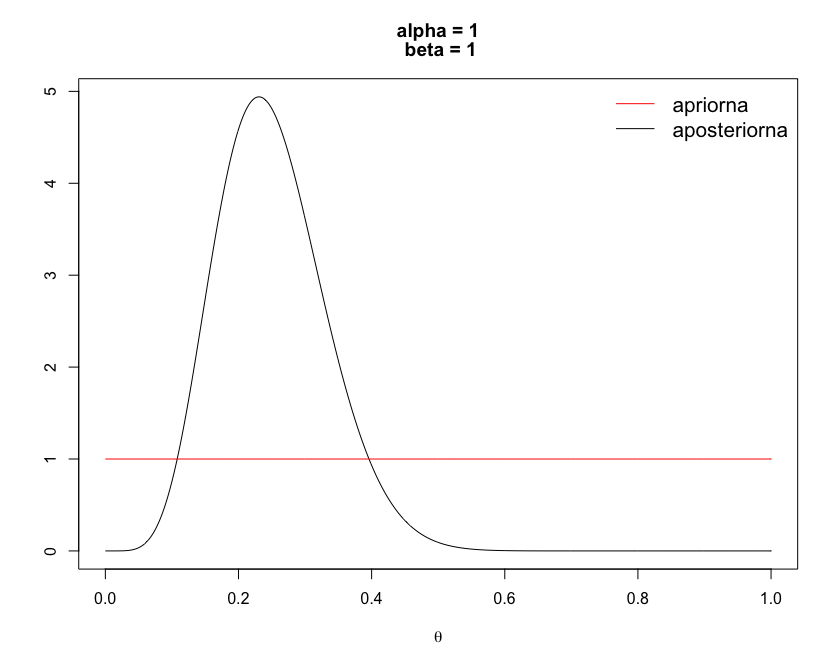
\includegraphics[width = 120mm]{Slike/1_3.png}
    \caption{Graf z apriorno in aposteriorno porazdelitev za $\alpha = \beta = 1$.}
\end{figure}

\begin{figure}[ht!]
    \begin{minipage}{0.5\textwidth}
        \centering
        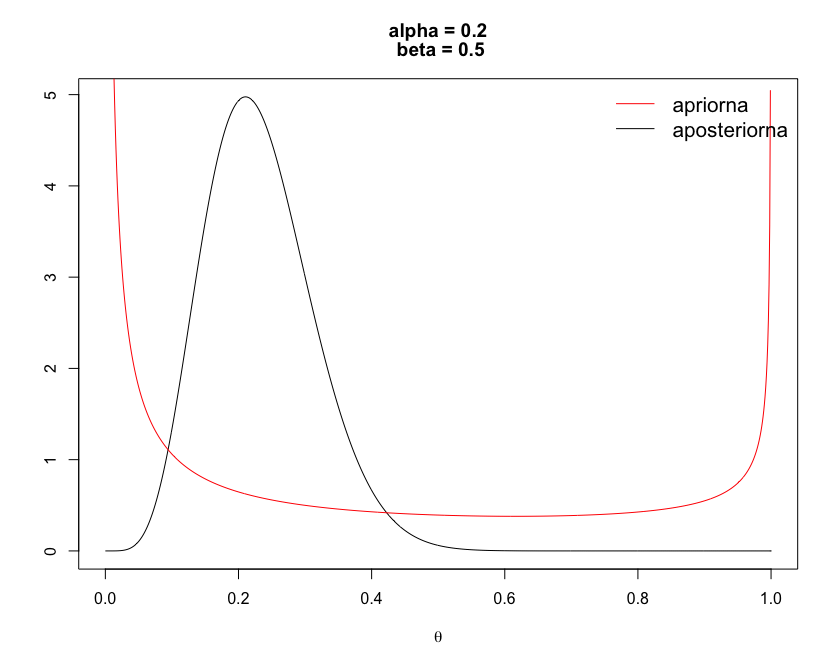
\includegraphics[width=82mm]{Slike/1_1.png}
    \end{minipage}\hfill
    \begin{minipage}{0.5\textwidth}
        \centering
        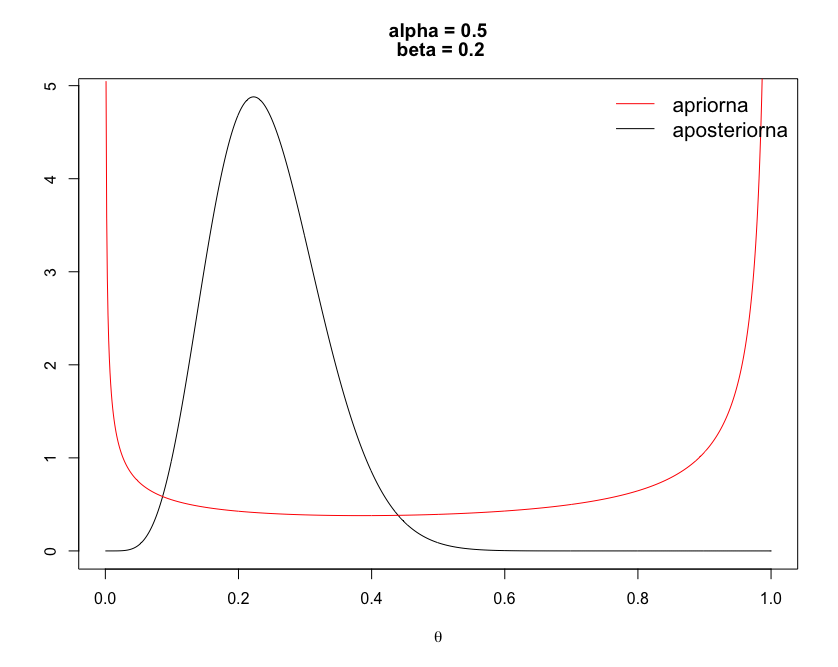
\includegraphics[width=82mm]{Slike/1_2.png}
    \end{minipage}\hfill
    \caption{Grafa z apriorno in aposteriorno porazdelitvijo z vrednostma 0.2 in 0.5.}
\end{figure}

\begin{figure}[ht!]
    \begin{minipage}{0.5\textwidth}
        \centering
        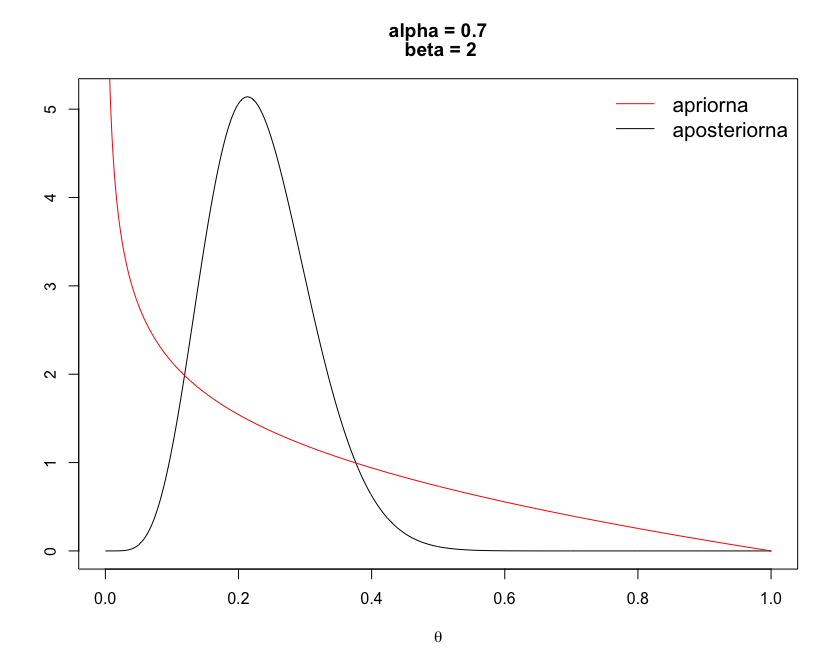
\includegraphics[width=82mm]{Slike/1_4.png}
    \end{minipage}\hfill
    \begin{minipage}{0.5\textwidth}
        \centering
        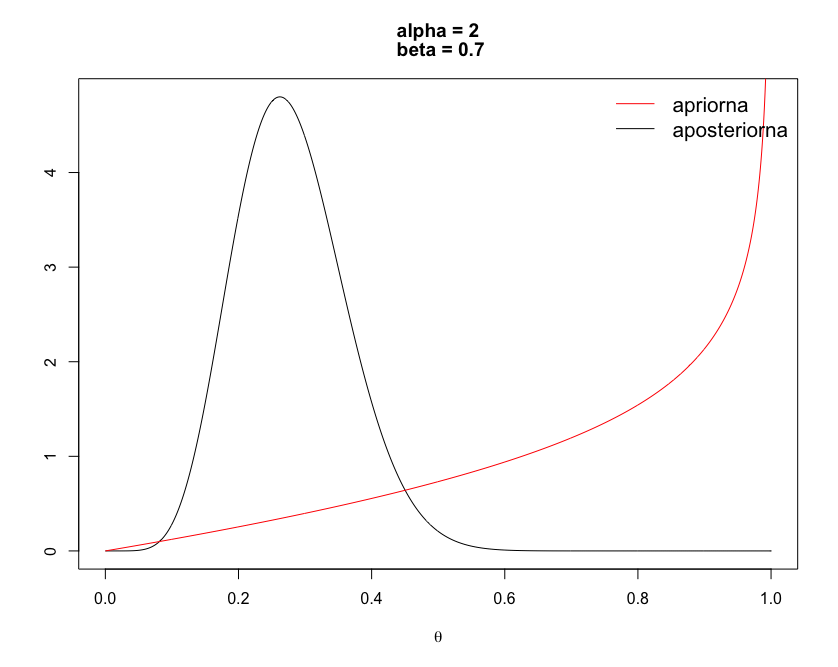
\includegraphics[width=82mm]{Slike/1_5.png}
    \end{minipage}\hfill
    \caption{Grafa z apriorno in aposteriorno porazdelitvijo z vrednostma 0.7 in 2.}
\end{figure}

\begin{figure}[ht!]
    \begin{minipage}{0.5\textwidth}
        \centering
        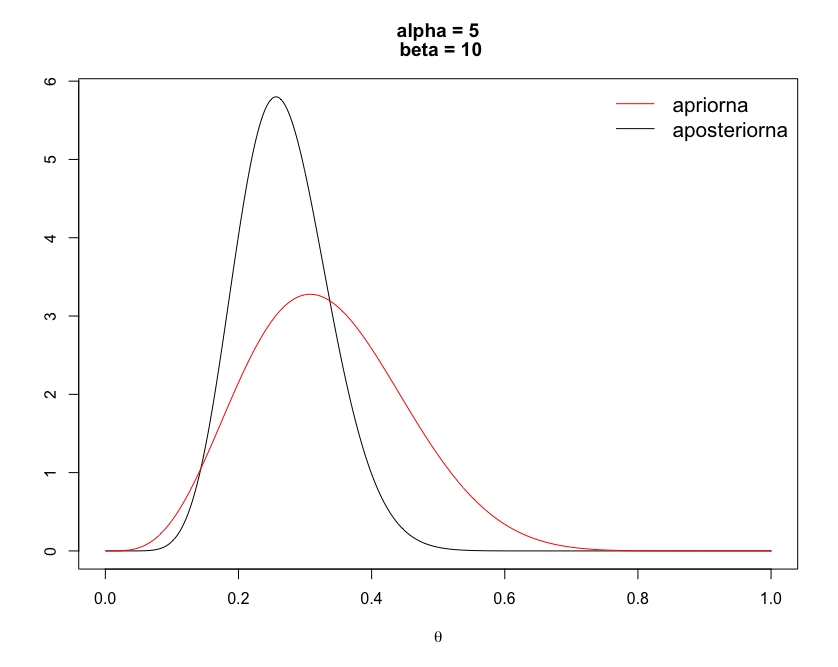
\includegraphics[width=82mm]{Slike/1_6.png}
    \end{minipage}\hfill
    \begin{minipage}{0.5\textwidth}
        \centering
        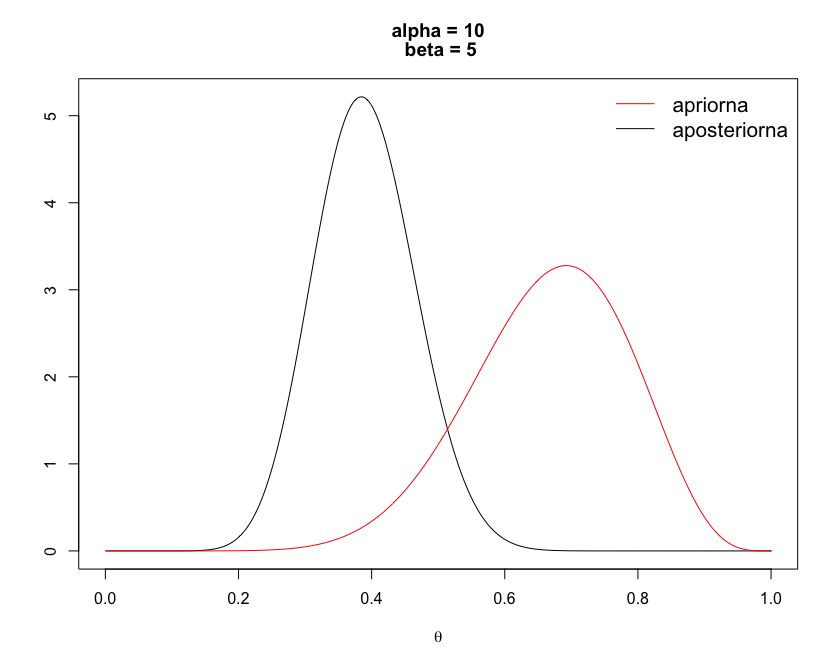
\includegraphics[width=82mm]{Slike/1_7.png}
    \end{minipage}\hfill
    \caption{Grafa z apriorno in aposteriorno porazdelitvijo z vrednostma 5 in 10.}
\end{figure}

\begin{figure}[ht!]
    \begin{minipage}{0.5\textwidth}
        \centering
        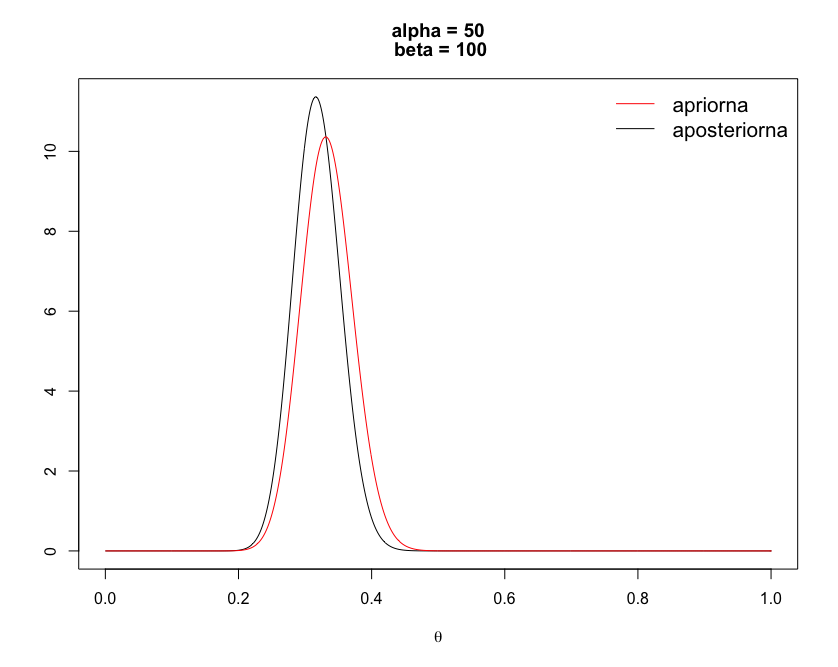
\includegraphics[width=82mm]{Slike/1_8.png}
    \end{minipage}\hfill
    \begin{minipage}{0.5\textwidth}
        \centering
        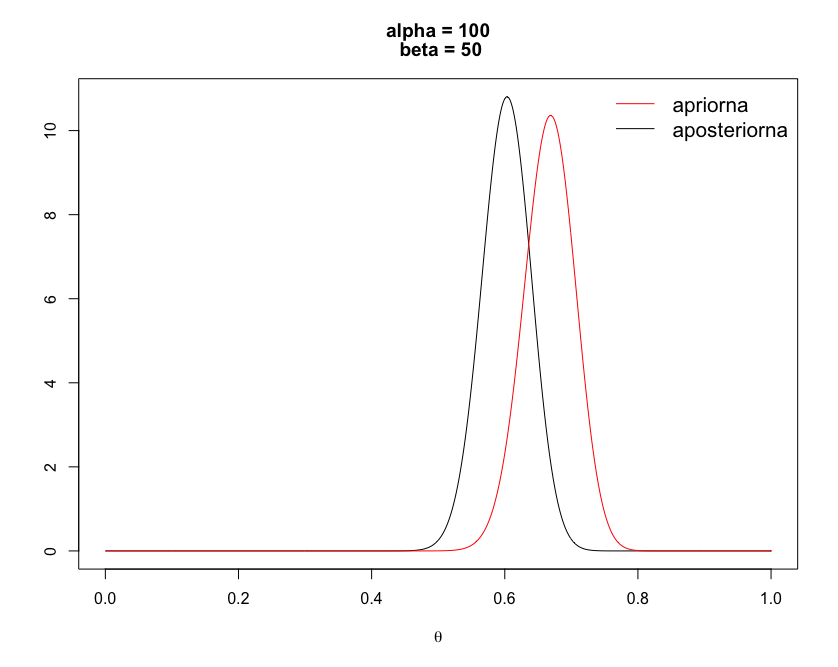
\includegraphics[width=82mm]{Slike/1_9.png}
    \end{minipage}\hfill
    \caption{Grafa z apriorno in aposteriorno porazdelitvijo z vrednostma 50 in 100.}
\end{figure}

\begin{figure}[ht!]
    \begin{minipage}{0.5\textwidth}
        \centering
        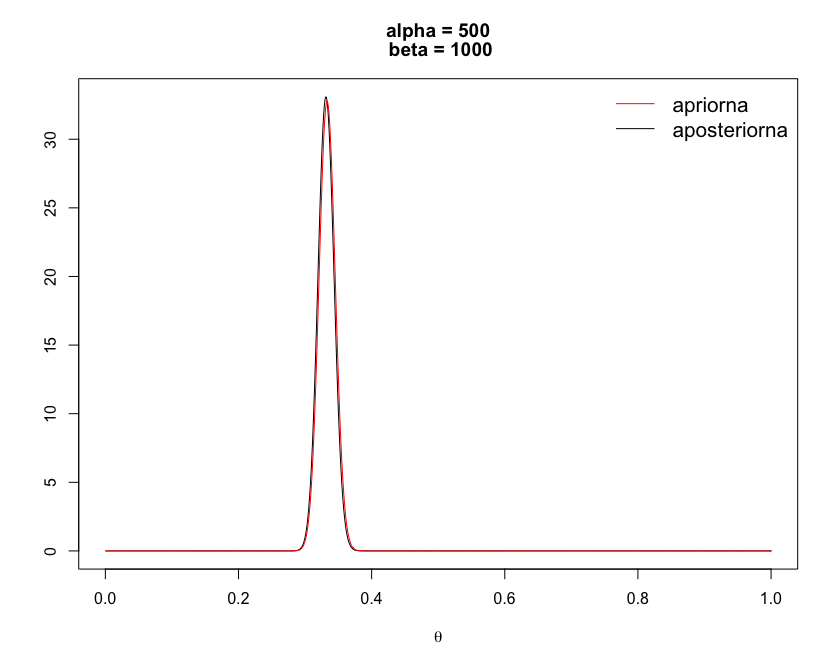
\includegraphics[width=82mm]{Slike/1_10.png}
    \end{minipage}\hfill
    \begin{minipage}{0.5\textwidth}
        \centering
        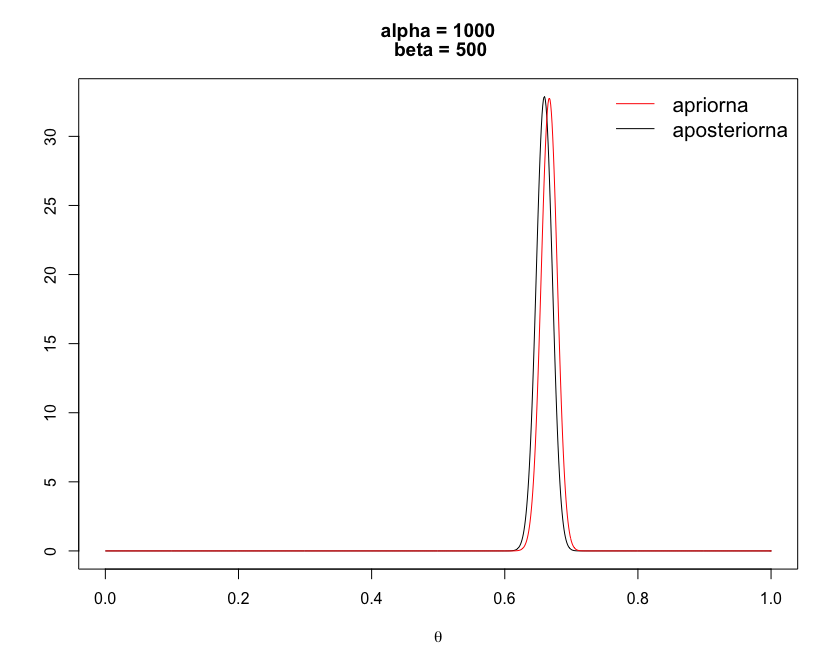
\includegraphics[width=82mm]{Slike/1_11.png}
    \end{minipage}\hfill
    \caption{Grafa z apriorno in aposteriorno porazdelitvijo z vrednostma 500 in 1000.}
\end{figure}

\newpage
Ugotovitve in opazke:
\begin{itemize}
    \item Za $\alpha$ in $\beta$ manjša od 1 je apriorna porazdelitev konveksne oblike.
    \item Če je ali $\alpha$ ali pa $\beta$ manjši od 1, predstavlja graf apriorne funkcije "polovico konveksne oblike" iz prejšnjega primera.
    \item Za $\alpha$ in $\beta$ večja od 1 je graf apriorne funkcije konkaven. 
    \item Graf aposteriorne funkcije je v vseh primerih konkaven.
    \item Hitro opazimo, da sta si grafa funkcij apriorne porazdelitve na levi in desni sliki v vsaki vrstici simetrični glede na os $x = 0.5$ (torej če zamenjamo vrednosti za $\alpha$ in $\beta$), 
aposterirno porazdelitev pa se, zaradi premika apriorne, zamakne v isto smer, kamor se preslika aposteriorna, torej v vseh teh primerih bolj v desno.
    \item Z večanjem $\alpha$ in $\beta$ hkrati opazimo, da sta si tudi obe porazdelitvi na grafu bližje (vrha sta vedno bolj "enotna"), saj na takšen način simuliramo večje zaupanje v predhodno znanje in bolj verjamemo apriorni porazdelitvi. 
    \item Podobno kot prej sta si z manjšanjem $\alpha$ in $\beta$ porazdelitvi na grafu različni in bolj narazen.
\end{itemize}

%%%%%%%%%%%%%%%%%%%%%%%%%%%%%%%%%%%%%%%%%%%%%%%%%%%%%%%%%%%%%%%%%%%%%%%%%%%%%%%%%%%%%%
\noindent
\textbf{2. naloga}
\\
Vemo, da je pričakovana vrednost apriorne porazdlitve enaka $0.25$ in v skladu s tem izberemo primerna $\alpha$ in $\beta$.
\\
Rešujemo torej enačbo z dvema neznankama
\begin{align*}
    E_{aprior} = \frac{1}{4} &= \frac{\alpha}{\alpha + \beta}
    \\
    \frac{1}{4} \alpha + \frac{1}{4} \beta &= \alpha
    \\
    \frac{1}{4} \beta &=\frac{3}{4} \alpha
    \\
    \beta &= 3 \alpha
\end{align*}
zato lahko parametra $\alpha$ in $\beta$ izberemo na neskončno načinov tako, da ustrezata linearni zvezi $ \beta = 3 \alpha$.
\\
Na spodnjih grafih je prikazanih nekaj takih možnosti za izbiro parametrov $\alpha$ in $\beta$.
\\
\\
Oceno pričakovane vrednosti lahko izrazimo kot pričakovano vrednost za aposteriorno porazdelitev: 
\begin{align*} 
    \frac{\alpha + k}{\alpha + k + \beta + n - k} &= \frac{\alpha + k}{\alpha + \beta + n} 
    \\
    &= \frac{(\alpha + \beta) \frac{\alpha}{\alpha + \beta} + n \frac{k}{n}}{\alpha + \beta + n}
    \\
    &= \frac{\alpha + \beta}{\alpha + \beta + n} \cdot \frac{\alpha}{\alpha + \beta} + \frac{n}{\alpha + \beta + n} \cdot \frac{k}{n},
\end{align*}
kar je konveksna kombinacija števil $\frac{\alpha}{\alpha + \beta}$ in $\frac{k}{n}$.
\\
Spomnimo se, da je $E_{aprior} = \frac{\alpha}{\alpha + \beta}$, izraz $\frac{k}{n}$ pa predstavlja frekventistično oceno. Označimo $\gamma(\alpha, \beta) = \alpha + \beta$. Tedaj lahko zgornjo enačbo zapišemo kot
\begin{align*} 
    E_{apost} = \frac{\gamma(\alpha, \beta)}{\gamma(\alpha, \beta)+ n} \cdot E_{aprior} + \frac{n}{\gamma(\alpha, \beta)+ n} \cdot \frac{k}{n}
\end{align*}

\newpage
\begin{figure}[ht!]
    \begin{minipage}{0.33\textwidth}
        \centering
        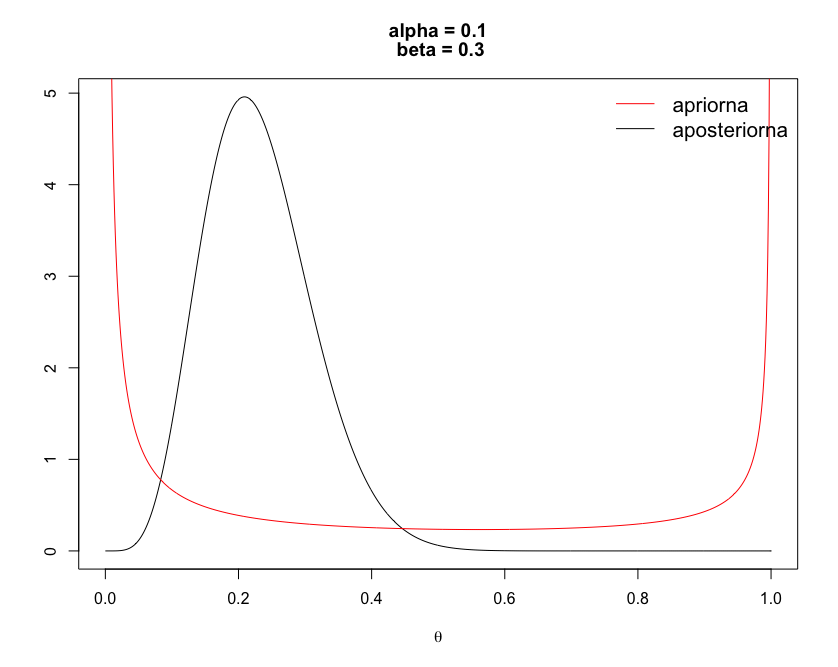
\includegraphics[width=55mm]{Slike/2_1.png}
    \end{minipage}\hfill
    \begin{minipage}{0.33\textwidth}
        \centering
        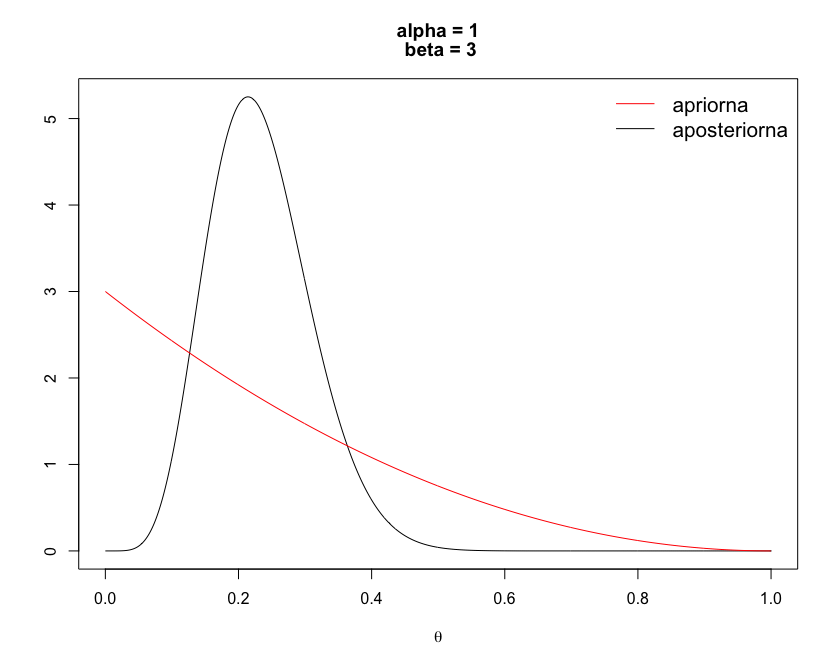
\includegraphics[width=55mm]{Slike/2_4.png}
    \end{minipage}\hfill
    \begin{minipage}{0.33\textwidth}
        \centering
        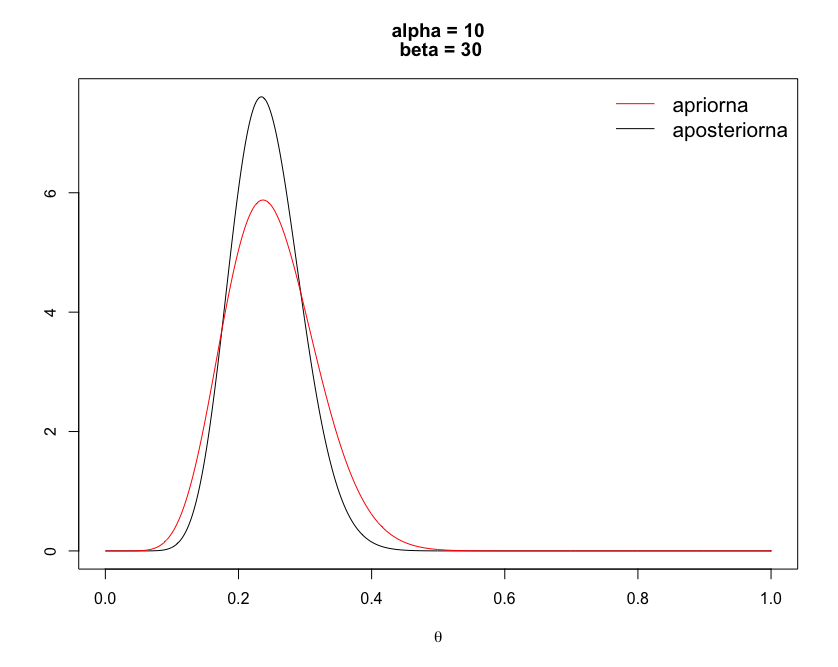
\includegraphics[width=55mm]{Slike/2_7.png}
    \end{minipage}\hfill
    \caption{Grafi z apriorno in aposteriorno porazdelitvijo za parametra, ki zadoščata  $\beta = 3 \alpha$.}
\end{figure}
\noindent
Ocene pričakovanih vrednosti za vse tri grafe, po vrsti:
\\
\texttt{[1] 0.2310606}
\\
\texttt{[2] 0.2333333}
\\
\texttt{[3] 0.2424242}

\begin{figure}[ht!]
    \begin{minipage}{0.33\textwidth}
        \centering
        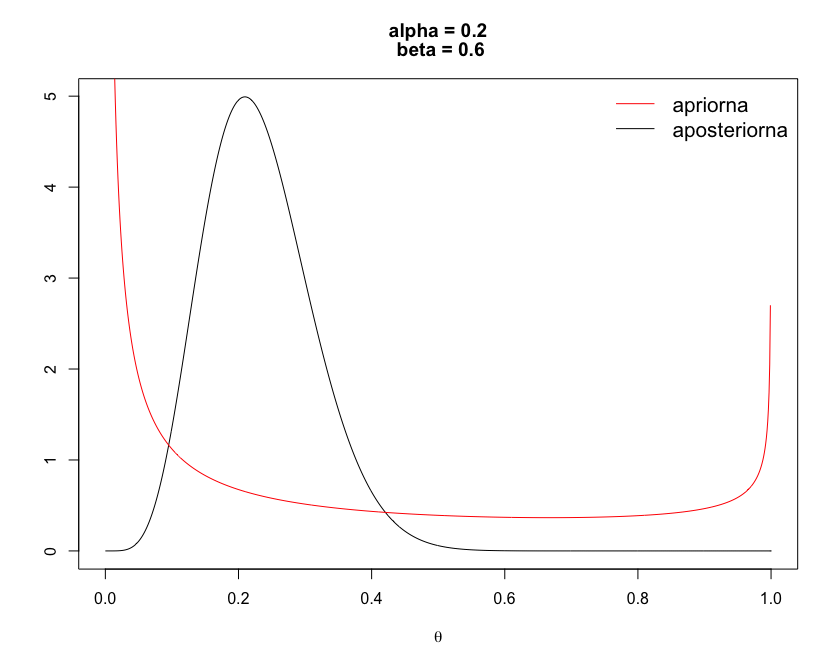
\includegraphics[width=55mm]{Slike/2_2.png}
    \end{minipage}\hfill
    \begin{minipage}{0.33\textwidth}
        \centering
        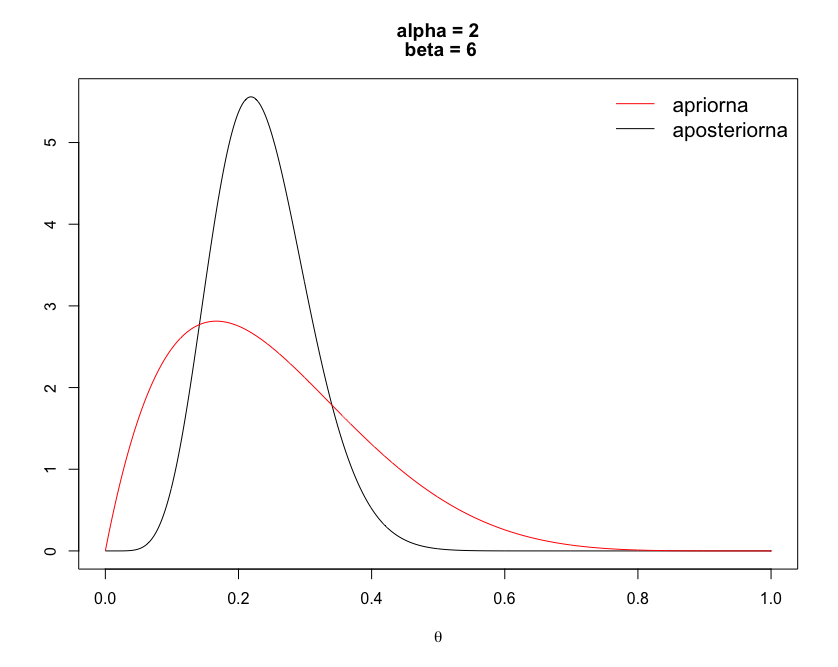
\includegraphics[width=55mm]{Slike/2_5.png}
    \end{minipage}\hfill
    \begin{minipage}{0.33\textwidth}
        \centering
        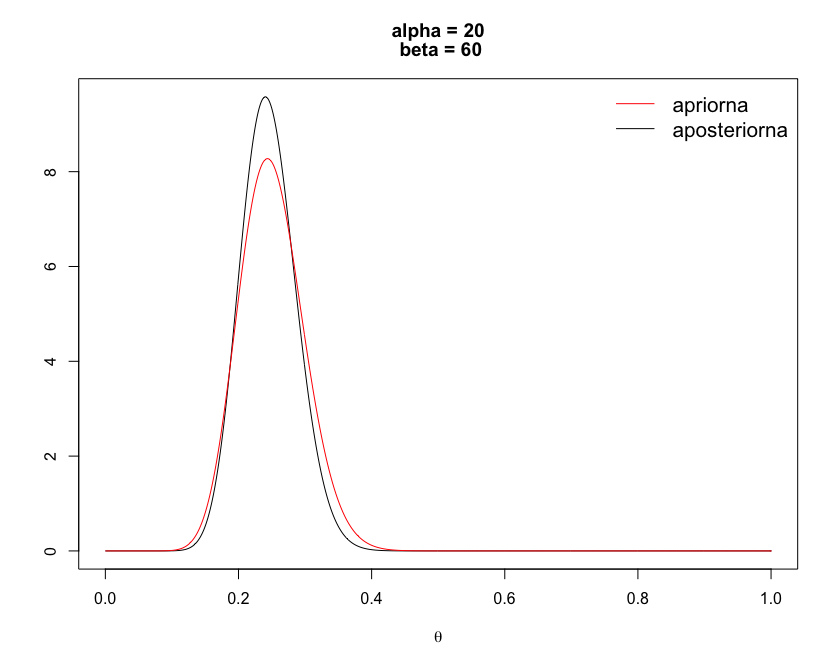
\includegraphics[width=55mm]{Slike/2_8.png}
    \end{minipage}\hfill
    \caption{Grafi z apriorno in aposteriorno porazdelitvijo za parametra, ki zadoščata  $\beta = 3 \alpha$.}
\end{figure}
\noindent
Ocene pričakovanih vrednosti za vse tri grafe, po vrsti:
\\
\texttt{[1] 0.2313433}
\\
\texttt{[2] 0.2352941}
\\
\texttt{[3] 0.245283}

\begin{figure}[ht!]
    \begin{minipage}{0.33\textwidth}
        \centering
        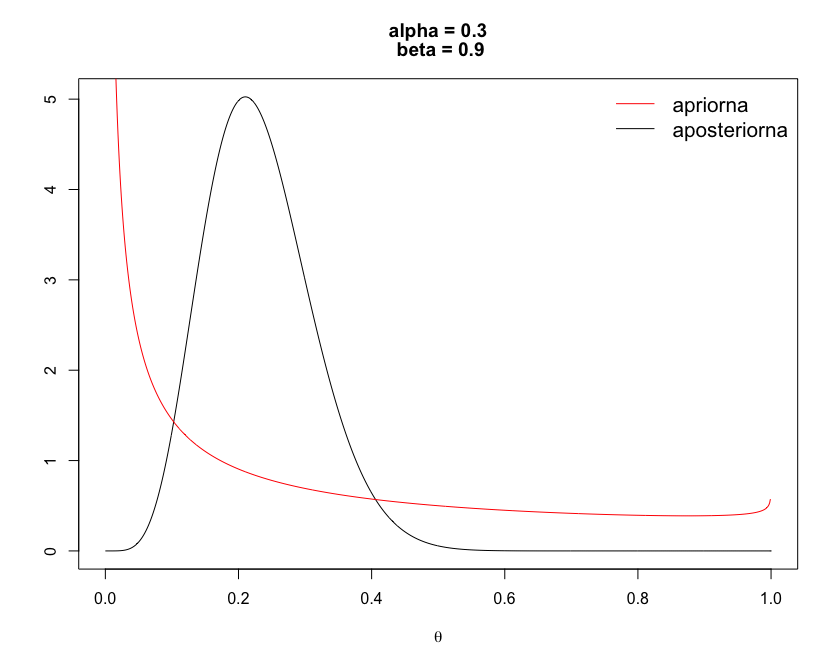
\includegraphics[width=55mm]{Slike/2_3.png}
    \end{minipage}\hfill
    \begin{minipage}{0.33\textwidth}
        \centering
        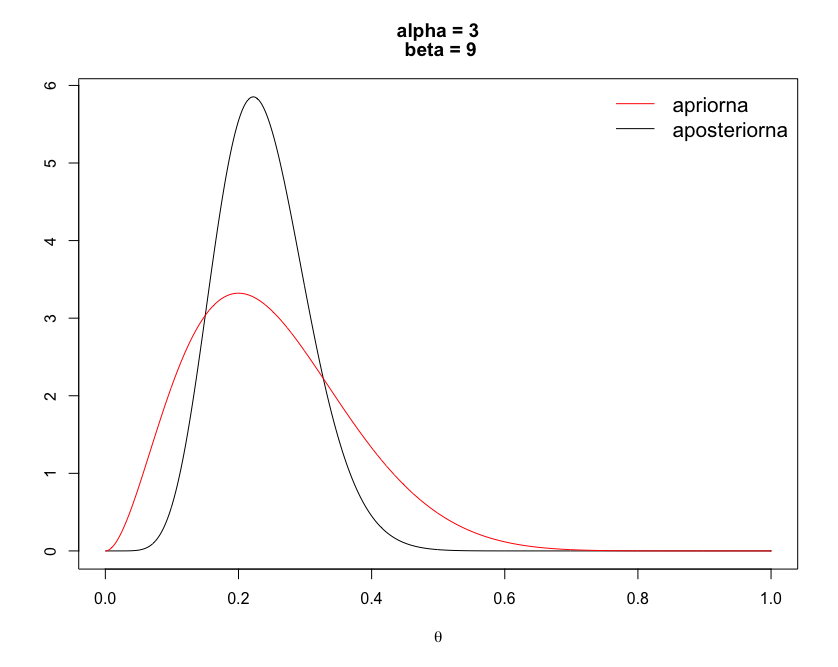
\includegraphics[width=55mm]{Slike/2_6.png}
    \end{minipage}\hfill
    \begin{minipage}{0.33\textwidth}
        \centering
        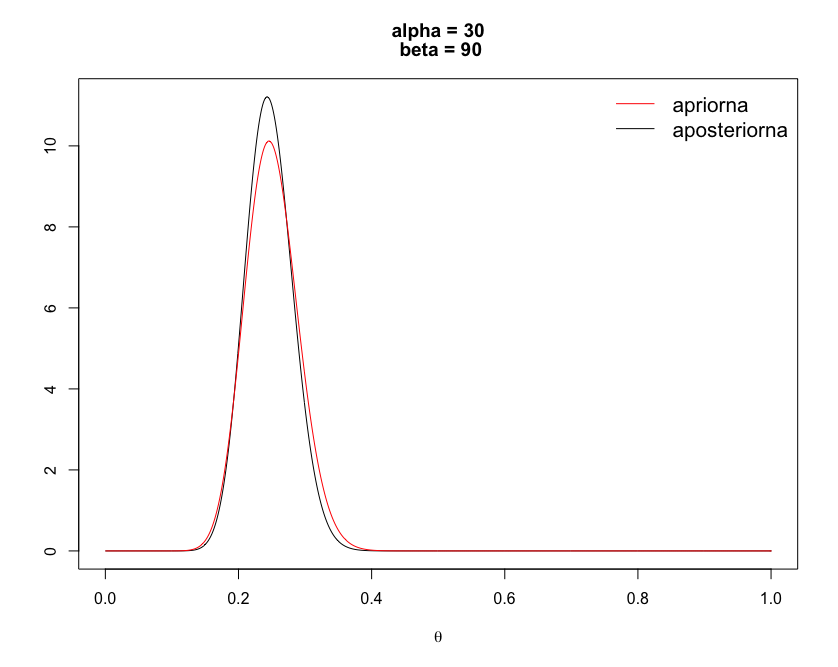
\includegraphics[width=55mm]{Slike/2_9.png}
    \end{minipage}\hfill
    \caption{Grafi z apriorno in aposteriorno porazdelitvijo za parametra, ki zadoščata  $\beta = 3 \alpha$.}
\end{figure}
Ocene pričakovanih vrednosti za vse tri grafe, po vrsti:
\\
\texttt{[1] 0.2316176}
\\
\texttt{[2] 0.2368421}
\\
\texttt{[3] 0.2465753}
\\
\\
Nadalje opazimo, da s funkcijo $\gamma(\alpha, \beta)$ kalibriramo verjetje v apriorno porazdelitev: z večanjem $\gamma(\alpha, \beta)$ bolj verjamemo apriorni porazdelitvi (takrat je manjša disperzija). 
Konkretno za ta primer: z večanjem $\gamma(\alpha, \beta)$ se ocena približuje vrednosti $\frac{1}{4} = 0.25$. To je razvidno tudi iz priloženih grafov.
\\

%%%%%%%%%%%%%%%%%%%%%%%%%%%%%%%%%%%%%%%%%%%%%%%%%%%%%%%%%%%%%%%%%%%%%%%%%%%%%%%%%%%%%%

\noindent
\textbf{3. naloga}
\\
Vzemimo sedaj vzorec študentov velikosti 30 izmed katerih jih je 21 odgovorilo pravilno. Privzamemo apriorno porazdelitev \texttt{Beta(1, 1)} in izračunajmo aposteriorno porazdelitev.
Prikažimo jo na grafu.

\begin{figure}[ht!]
    \centering
    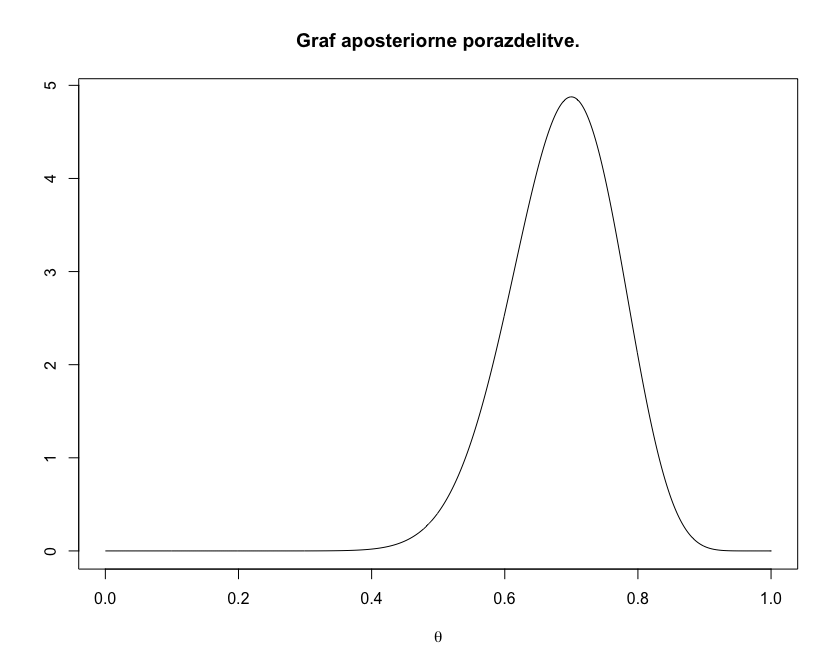
\includegraphics[width = 120mm]{Slike/3.png}
    \caption{Graf aposteriorne porazdelitve pri danih podatkih.}
\end{figure}

%%%%%%%%%%%%%%%%%%%%%%%%%%%%%%%%%%%%%%%%%%%%%%%%%%%%%%%%%%%%%%%%%%%%%%%%%%%%%%%%%%%%%%

\noindent
\textbf{4. naloga}
\\
Primerjajmo aposteriorno porazdelitev iz naloge 3, označimo jo $Z_1$, z aposteriorno porazdelitvijo porazdelitve \texttt{Beta(7, 21)}, ki smo jo izračunali na vajah.
Ocenimo verjetnost $P(Z_2 < Z_1)$.
\\
Ocenjeno verjetnost izračunamo s cenilko na tak način, da primerjamo $Z_1$ in $Z_2$ po elementih. Natančneje, za vsak istoležni element preverimo ali je element iz porazdelitve $Z_2$ manjši od elementa iz porazdelitve $Z_1$. 
Vsoto oz. seštevek za ta pogoj na koncu delimo s 10000 (toliko kot je generiranih vrednosti v obeh porazdelitvah). 
\\
Ocenjena verjetnost znaša: 
\\
\textttt{[1] 0.9998}
\\
Na podlagi simulacije izračunajmo še $95\%$ interval zaupanja, poročamo kar $2.5\%$ in $97.5\%$ kvantil simuliranih podatkov.
\\
Izračunajmo najprej interval zaupanja za vsako od obeh aposteriornih porazdelitev.
\\
\texttt{
$Z_1$: 
\\
2.5\%     97.5\% 
\\
0.5214762 0.8337051 
\\
$Z_2$: 
\\
2.5\%     97.5\% 
\\
0.1110932 0.4164294 
}
\\
\\
Za interval zaupanja na podlagi simulacije za primerjanje obeh porazdelite vzamemo kar razliko (po komponentah) vektorjev s 10000 generiranimi vrednostmi iz obeh aposteriornih porazdelitev,
kar je sorodno zgornji cenilki, s pomočjo katere smo prišli do ocene verjetnosti.
Dobimo: 
\\
\texttt{
2.5\%     97.5\% 
\\
0.2024990 0.6452275 
}





\end{document}

\begin{thebibliography}{99}

\end{thebibliography}